% Options for packages loaded elsewhere
\PassOptionsToPackage{unicode}{hyperref}
\PassOptionsToPackage{hyphens}{url}
%
\documentclass[
  english,
  man,floatsintext]{apa6}
\usepackage{lmodern}
\usepackage{amssymb,amsmath}
\usepackage{ifxetex,ifluatex}
\ifnum 0\ifxetex 1\fi\ifluatex 1\fi=0 % if pdftex
  \usepackage[T1]{fontenc}
  \usepackage[utf8]{inputenc}
  \usepackage{textcomp} % provide euro and other symbols
\else % if luatex or xetex
  \usepackage{unicode-math}
  \defaultfontfeatures{Scale=MatchLowercase}
  \defaultfontfeatures[\rmfamily]{Ligatures=TeX,Scale=1}
\fi
% Use upquote if available, for straight quotes in verbatim environments
\IfFileExists{upquote.sty}{\usepackage{upquote}}{}
\IfFileExists{microtype.sty}{% use microtype if available
  \usepackage[]{microtype}
  \UseMicrotypeSet[protrusion]{basicmath} % disable protrusion for tt fonts
}{}
\makeatletter
\@ifundefined{KOMAClassName}{% if non-KOMA class
  \IfFileExists{parskip.sty}{%
    \usepackage{parskip}
  }{% else
    \setlength{\parindent}{0pt}
    \setlength{\parskip}{6pt plus 2pt minus 1pt}}
}{% if KOMA class
  \KOMAoptions{parskip=half}}
\makeatother
\usepackage{xcolor}
\IfFileExists{xurl.sty}{\usepackage{xurl}}{} % add URL line breaks if available
\IfFileExists{bookmark.sty}{\usepackage{bookmark}}{\usepackage{hyperref}}
\hypersetup{
  pdftitle={Identifying Factors That Affect Political Freedom Within the OECD},
  pdfauthor={Joe Despres1, Sabrina Ball1, Jacob Haywood1, \& Joe Sigler1},
  pdflang={en-EN},
  pdfkeywords={keywords},
  hidelinks,
  pdfcreator={LaTeX via pandoc}}
\urlstyle{same} % disable monospaced font for URLs
\usepackage{graphicx}
\makeatletter
\def\maxwidth{\ifdim\Gin@nat@width>\linewidth\linewidth\else\Gin@nat@width\fi}
\def\maxheight{\ifdim\Gin@nat@height>\textheight\textheight\else\Gin@nat@height\fi}
\makeatother
% Scale images if necessary, so that they will not overflow the page
% margins by default, and it is still possible to overwrite the defaults
% using explicit options in \includegraphics[width, height, ...]{}
\setkeys{Gin}{width=\maxwidth,height=\maxheight,keepaspectratio}
% Set default figure placement to htbp
\makeatletter
\def\fps@figure{htbp}
\makeatother
\setlength{\emergencystretch}{3em} % prevent overfull lines
\providecommand{\tightlist}{%
  \setlength{\itemsep}{0pt}\setlength{\parskip}{0pt}}
\setcounter{secnumdepth}{-\maxdimen} % remove section numbering
% Make \paragraph and \subparagraph free-standing
\ifx\paragraph\undefined\else
  \let\oldparagraph\paragraph
  \renewcommand{\paragraph}[1]{\oldparagraph{#1}\mbox{}}
\fi
\ifx\subparagraph\undefined\else
  \let\oldsubparagraph\subparagraph
  \renewcommand{\subparagraph}[1]{\oldsubparagraph{#1}\mbox{}}
\fi
% Manuscript styling
\usepackage{upgreek}
\captionsetup{font=singlespacing,justification=justified}

% Table formatting
\usepackage{longtable}
\usepackage{lscape}
% \usepackage[counterclockwise]{rotating}   % Landscape page setup for large tables
\usepackage{multirow}		% Table styling
\usepackage{tabularx}		% Control Column width
\usepackage[flushleft]{threeparttable}	% Allows for three part tables with a specified notes section
\usepackage{threeparttablex}            % Lets threeparttable work with longtable

% Create new environments so endfloat can handle them
% \newenvironment{ltable}
%   {\begin{landscape}\begin{center}\begin{threeparttable}}
%   {\end{threeparttable}\end{center}\end{landscape}}
\newenvironment{lltable}{\begin{landscape}\begin{center}\begin{ThreePartTable}}{\end{ThreePartTable}\end{center}\end{landscape}}

% Enables adjusting longtable caption width to table width
% Solution found at http://golatex.de/longtable-mit-caption-so-breit-wie-die-tabelle-t15767.html
\makeatletter
\newcommand\LastLTentrywidth{1em}
\newlength\longtablewidth
\setlength{\longtablewidth}{1in}
\newcommand{\getlongtablewidth}{\begingroup \ifcsname LT@\roman{LT@tables}\endcsname \global\longtablewidth=0pt \renewcommand{\LT@entry}[2]{\global\advance\longtablewidth by ##2\relax\gdef\LastLTentrywidth{##2}}\@nameuse{LT@\roman{LT@tables}} \fi \endgroup}

% \setlength{\parindent}{0.5in}
% \setlength{\parskip}{0pt plus 0pt minus 0pt}

% Overwrite redefinition of paragraph and subparagraph by the default LaTeX template
% See https://github.com/crsh/papaja/issues/292
\makeatletter
\renewcommand{\paragraph}{\@startsection{paragraph}{4}{\parindent}%
  {0\baselineskip \@plus 0.2ex \@minus 0.2ex}%
  {-1em}%
  {\normalfont\normalsize\bfseries\itshape\typesectitle}}

\renewcommand{\subparagraph}[1]{\@startsection{subparagraph}{5}{1em}%
  {0\baselineskip \@plus 0.2ex \@minus 0.2ex}%
  {-\z@\relax}%
  {\normalfont\normalsize\itshape\hspace{\parindent}{#1}\textit{\addperi}}{\relax}}
\makeatother

% \usepackage{etoolbox}
\makeatletter
\patchcmd{\HyOrg@maketitle}
  {\section{\normalfont\normalsize\abstractname}}
  {\section*{\normalfont\normalsize\abstractname}}
  {}{\typeout{Failed to patch abstract.}}
\patchcmd{\HyOrg@maketitle}
  {\section{\protect\normalfont{\@title}}}
  {\section*{\protect\normalfont{\@title}}}
  {}{\typeout{Failed to patch title.}}
\makeatother
\shorttitle{RUNNING HEAD: Political Freedom Within the OECD}
\keywords{keywords\newline\indent Word count: X}
\usepackage{lineno}

\linenumbers
\usepackage{csquotes}
\ifxetex
  % Load polyglossia as late as possible: uses bidi with RTL langages (e.g. Hebrew, Arabic)
  \usepackage{polyglossia}
  \setmainlanguage[]{english}
\else
  \usepackage[shorthands=off,main=english]{babel}
\fi
\newlength{\cslhangindent}
\setlength{\cslhangindent}{1.5em}
\newenvironment{cslreferences}%
  {\setlength{\parindent}{0pt}%
  \everypar{\setlength{\hangindent}{\cslhangindent}}\ignorespaces}%
  {\par}

\title{Identifying Factors That Affect Political Freedom Within the OECD}
\author{Joe Despres\textsuperscript{1}, Sabrina Ball\textsuperscript{1}, Jacob Haywood\textsuperscript{1}, \& Joe Sigler\textsuperscript{1}}
\date{Last compiled 18:41}


\affiliation{\vspace{0.5cm}\textsuperscript{1} Michigan State University}

\begin{document}
\maketitle

\hypertarget{introduction}{%
\subsection{Introduction}\label{introduction}}

2020 is an election year, which has many of use reflecting on political freedoms. Political freedoms are important because they have a dramatic impact on the quality of life for the citizens of a country. Such reflection has us asking: What factors are associated with an increase in political freedom around the world? Political freedom is an abstract concept that does not lend well to quantification. However, Freedom House (\emph{Countries and Territories}, 2020), a U.S. based think tank and research institute, attempts this by assigning a index of political rights to each country every year based on a fixed criteria.

The Political Rights Index is comprised of three subcategories. Electoral process, political participation, and functioning government. Electoral process is a score based on how the current government leaders were selected. How fairly the positions was obtained and kept. As well as the fairness of the current electoral laws, how they are implemented and the degree to which there is an independent judiciary. Political Participation is evaluated on four criteria, right to form parties, realistic opposition to current power, political choice free from military, religious powers, economic oligarchies, or any other unaccountable body, and various minority groups having full political rights. Functioning government, is the current heads of government determine policies, safeguards against corruption, and openness and transparency of government operation. Political freedom has been measured in this manner for every country from the years 1978 to present.

Although such a metric is far from perfect. This will serve as a reasonable measure of political freedom around the world and will serve as an adequate sample to study political freedom. We obtained this from the Gapminder Foundation Rosling (2020), a non-profit organization that studies and promotes economic development. After carefully selecting a dependent variable, we browsed data that were also available from Gapminder and selected variables that we felt would be helpful in explaining political freedom in various countries. To explain a country's political rights index we selected: Corruption Perception Index, Education Expenditure, Electricity Use, Gini Coefficient, Internet Users as a percentage, Labor Force Participation Rate, Military Spending as percentage of GDP, and Murders per million.

\hypertarget{data}{%
\subsection{Data}\label{data}}

These data sets were separate so we downloaded them individually, cleaned and combined them together using R R Core Team (2020) and the Tidyverse Package Wickham et al. (2019). This resulted in a data set with all 196 countries form years 1950 to 2030 (data after 2019 were projections). It was immediately apparent that there was a substantial amount of missing data in an obvious pattern. Less developed countries tended to have more missing data points. Also, the further back in time the more missing data points. Had we conducted this study as it was it would have been severely biased towards more developed countries as missing data points would be dropped. This forced us to narrow the scope of the study and focus only on countries within the Organization for Economic Co-operation and Development (OECD). This subset of countries has a reasonably complete data. Therefore, we removed data from countries that are not members of the OECD and selected only the years 2000 through 2018.

This remedied most of the missing datapoints. However, even within the OEDC there were sparse few missing data points. From there, we imputed the median of each country's variable. For instance, Austria's electricity consumption was missing for 2012, so we took the median of Austria's consumption over the 18 year period. Which afforded us the ability to keep even more data with minimal compromise. This is a reasonable procedure because the covariates do not fluctuate wildly year over year. After that, there were a few other cases which we needed to input manually, for example, Iceland's Military spending is 0\% of their GDP, so we replaced the NA with a 0. This afforded us a full data set with no missing data points.

\hypertarget{descriptive-statistics}{%
\subsection{Descriptive Statistics}\label{descriptive-statistics}}

\begin{longtable}[t]{lrrrrrr}
\caption{\label{tab:unnamed-chunk-1}Descriptive Statistics}\\
\toprule
Variable & Mean & Median & Std & Min & Max & Range\\
\midrule
Political Rights & 6.60 & 7.00 & 0.79 & 2.00 & 7.00 & 5.00\\
Year & 2009.50 & 2009.50 & 5.19 & 2001.00 & 2018.00 & 17.00\\
Corruption Perception & 31.95 & 29.00 & 15.87 & 8.00 & 71.00 & 63.00\\
Education Expenditure & 0.20 & 0.20 & 0.04 & 0.10 & 0.37 & 0.27\\
Electricity Use & 8682.17 & 6695.00 & 7533.32 & 866.00 & 54800.00 & 53934.00\\
\addlinespace
Gini & 33.77 & 32.70 & 6.35 & 24.40 & 56.80 & 32.40\\
Internet Users & 65.41 & 70.90 & 22.93 & 2.85 & 99.00 & 96.15\\
Life Expectancy & 0.60 & 0.61 & 0.06 & 0.45 & 0.78 & 0.33\\
Labor Force Participation & 79.30 & 80.00 & 2.84 & 70.20 & 84.40 & 14.20\\
Military Spending & 1.68 & 1.41 & 1.16 & 0.00 & 8.54 & 8.54\\
\addlinespace
Murders rate & 3.13 & 1.04 & 6.15 & 0.15 & 29.07 & 28.92\\
\bottomrule
\end{longtable}

Table 1 made with the Zhu (2020) contains Basic summary statistics from our dataset. We observe that the mean political rights is 6.6 nearly full with a fairly low standard deviation. This is not ideal. We would much prefer that it was continuous with a substantial variation. First, the methodology of rather than taking continuous values Freedomhouse's classification is discrete classifying countries political rights taking values of the integers 1-7. Secondly countries with a low political rights by nature have a suspect data reporting process. Which is why we had to select a subset of countries and that subset leans towards having more political freedom. We precede on the understanding that there are moderate problems with the data, first having a discrete response variable and the nature of the distribution being skewed towards the maximum 7/7 political freedom.

With such considerations taken into account, we will not be making any non-linear transformation or variables. First, we examined the results of that we did not find compelling evidence to support making a such a transformation and the data are roughly linear. With a clean, complete, and dataset that is contains flaws but is still reasonably holds assumptions we performed the best subsection algorithm to obtain a model with the best fit. This lead us to choose between the following models. From the graph of the subsets we can see that the increase in \(R^2\) and \(AIC\) by adding additional paramaters.

\begin{figure}
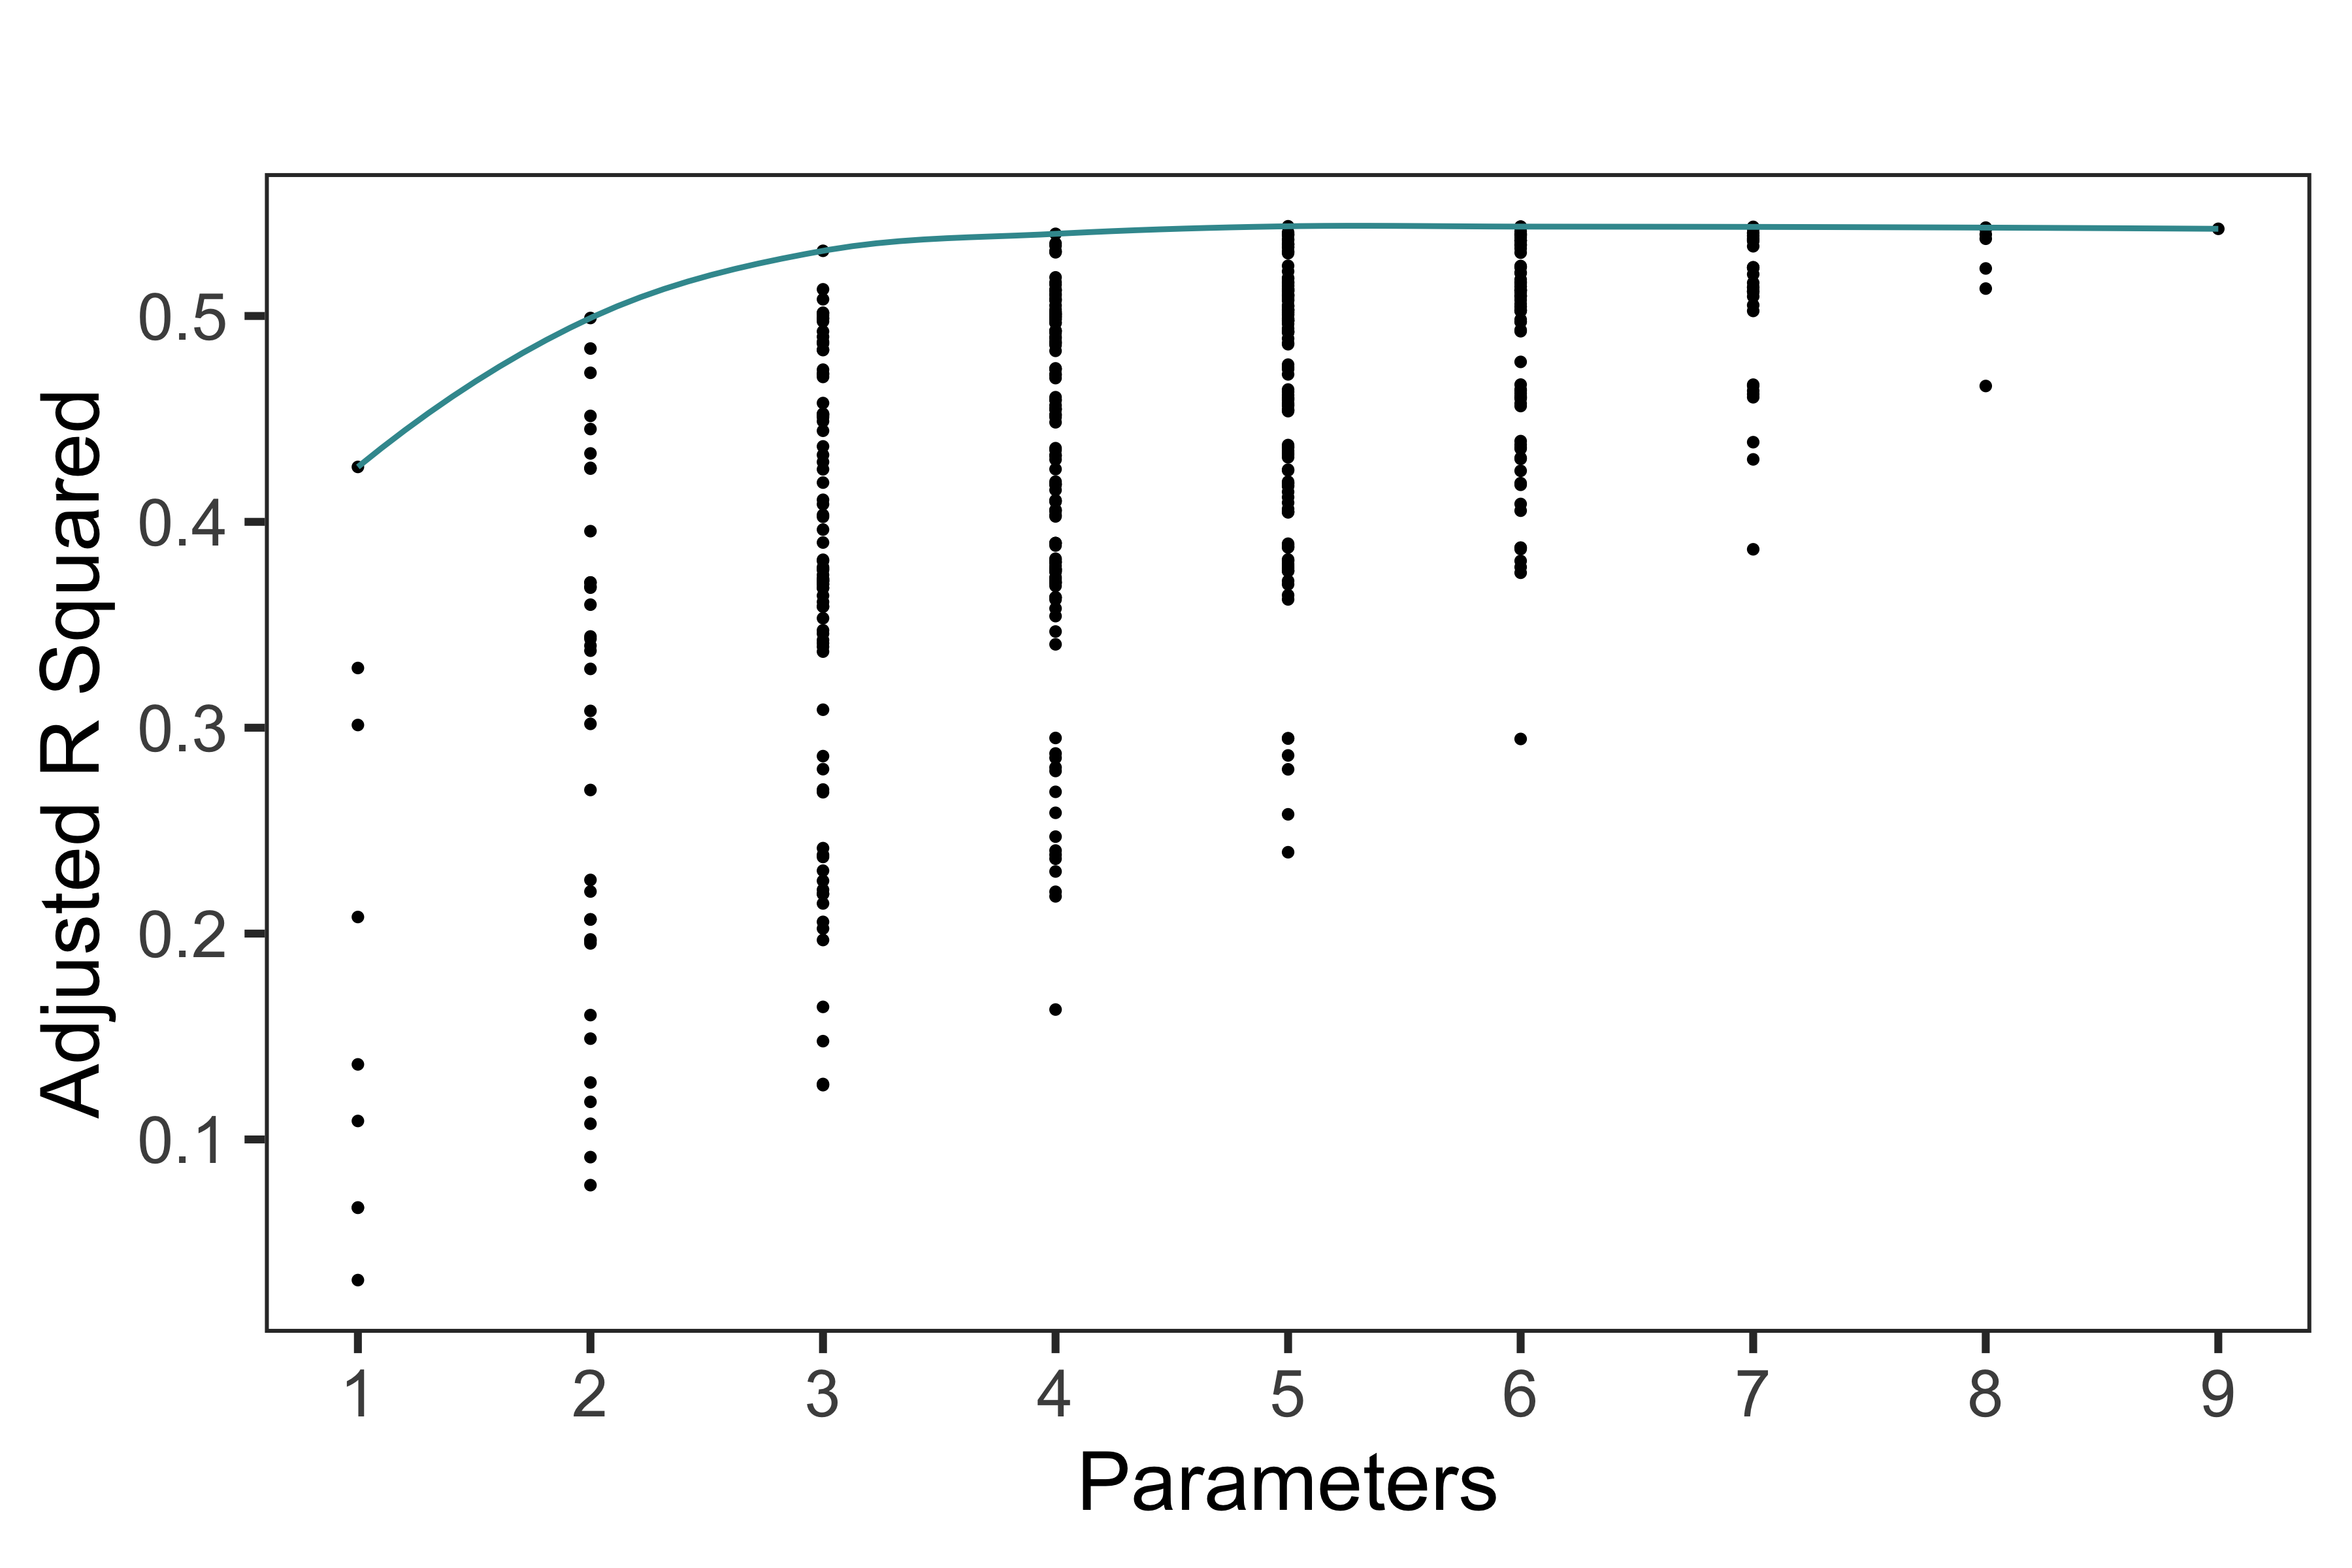
\includegraphics[width=0.5\linewidth]{paper_files/figure-latex/unnamed-chunk-2-1} 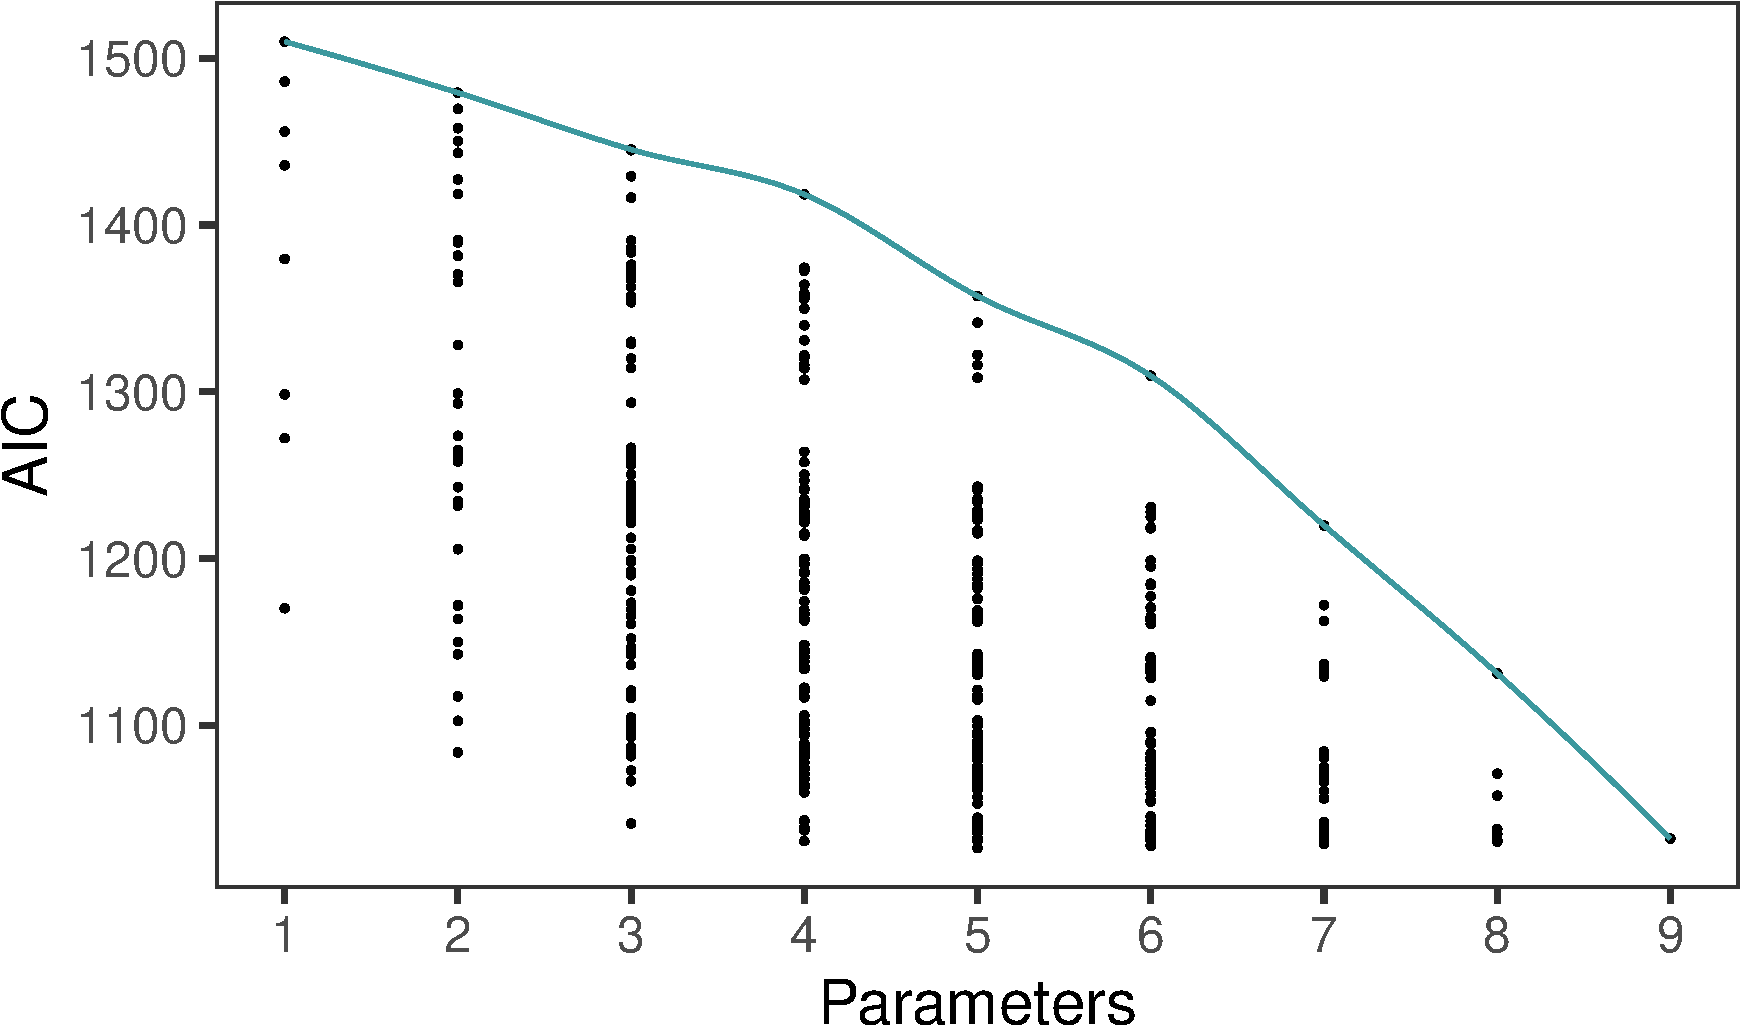
\includegraphics[width=0.5\linewidth]{paper_files/figure-latex/unnamed-chunk-2-2} \caption{ }\label{fig:unnamed-chunk-2}
\end{figure}

\hypertarget{model}{%
\subsection{Model}\label{model}}

\(\operatorname{polrights\_fh} = \beta_{0} + \beta_{1}(\operatorname{corruption\_perception\_index\_cpi}) + \beta_{2}(\operatorname{edu\_exp\_gdp\_per\_person}) + \beta_{3}(\operatorname{life\_expectancy\_years}) + \beta_{4}(\operatorname{military\_spending\_pct\_of\_gdp}) + \beta_{5}(\operatorname{murder\_per\_mil\_people}) + \epsilon\)

(chart here)

The model that displayed the most statistical sense in conjuction with our exsistin inutitions is.
(formula here)

\hypertarget{results}{%
\subsection{Results}\label{results}}

See table 1 made in stargazer Hlavac (2018)

\begin{table}[!htbp] \centering 
  \caption{Regression Results} 
  \label{} 
\begin{tabular}{@{\extracolsep{5pt}}lccc} 
\\[-1.8ex]\hline 
\hline \\[-1.8ex] 
 & \multicolumn{3}{c}{Political Rights Index} \\ 
\cline{2-4} 
 & DF = 6 & DF = 5 & DF = 4 \\ 
\hline \\[-1.8ex] 
 (Intercept) & $-$0.023$^{***}$ & $-$0.023$^{***}$ & $-$0.022$^{***}$ \\ 
  & (0.002) & (0.002) & (0.002) \\ 
  Corruption Perception & 1.746$^{***}$ & 1.900$^{***}$ & 1.898$^{***}$ \\ 
  & (0.562) & (0.534) & (0.536) \\ 
  Education Expendature & 0.001 &  &  \\ 
  & (0.001) &  &  \\ 
  Life Expectancy & $-$0.025$^{***}$ & $-$0.021$^{**}$ &  \\ 
  & (0.009) & (0.008) &  \\ 
  Military Spending & $-$0.146$^{***}$ & $-$0.150$^{***}$ & $-$0.153$^{***}$ \\ 
  & (0.019) & (0.019) & (0.019) \\ 
  Murder Rate & $-$0.035$^{***}$ & $-$0.035$^{***}$ & $-$0.033$^{***}$ \\ 
  & (0.004) & (0.004) & (0.004) \\ 
  Constant & 9.212$^{***}$ & 8.979$^{***}$ & 7.284$^{***}$ \\ 
  & (0.742) & (0.692) & (0.123) \\ 
 \hline \\[-1.8ex] 
Observations & 648 & 648 & 648 \\ 
R$^{2}$ & 0.548 & 0.547 & 0.543 \\ 
Adjusted R$^{2}$ & 0.543 & 0.544 & 0.540 \\ 
Residual Std. Error & 0.531 & 0.531 & 0.533 \\ 
F Statistic & 129.343$^{***}$ & 155.112$^{***}$ & 190.808$^{***}$ \\ 
\hline 
\hline \\[-1.8ex] 
\textit{Note:}  & \multicolumn{3}{r}{$^{*}$p$<$0.1; $^{**}$p$<$0.05; $^{***}$p$<$0.01} \\ 
\end{tabular} 
\end{table}

\hypertarget{remeidal-measures}{%
\subsection{Remeidal Measures}\label{remeidal-measures}}

\hypertarget{conclusion}{%
\subsection{Conclusion}\label{conclusion}}

\newpage

\hypertarget{references}{%
\section{References}\label{references}}

\begingroup
\setlength{\parindent}{-0.5in}
\setlength{\leftskip}{0.5in}

\hypertarget{refs}{}
\begin{cslreferences}
\leavevmode\hypertarget{ref-Freedomhouse}{}%
\emph{Countries and territories}. (2020). Washington D.C.: Freedomhouse. Retrieved from \url{https://freedomhouse.org}

\leavevmode\hypertarget{ref-R-stargazer}{}%
Hlavac, M. (2018). \emph{Stargazer: Well-formatted regression and summary statistics tables}. Bratislava, Slovakia: Central European Labour Studies Institute (CELSI). Retrieved from \url{https://CRAN.R-project.org/package=stargazer}

\leavevmode\hypertarget{ref-R-base}{}%
R Core Team. (2020). \emph{R: A language and environment for statistical computing}. Vienna, Austria: R Foundation for Statistical Computing. Retrieved from \url{https://www.R-project.org/}

\leavevmode\hypertarget{ref-Gapminder}{}%
Rosling, H. (2020). \emph{Gapminder}. Retrieved from \url{https://www.gapminder.org/data/}

\leavevmode\hypertarget{ref-R-tidyverse}{}%
Wickham, H., Averick, M., Bryan, J., Chang, W., McGowan, L. D., François, R., \ldots{} Yutani, H. (2019). Welcome to the tidyverse. \emph{Journal of Open Source Software}, \emph{4}(43), 1686. \url{https://doi.org/10.21105/joss.01686}

\leavevmode\hypertarget{ref-R-kableExtra}{}%
Zhu, H. (2020). \emph{KableExtra: Construct complex table with 'kable' and pipe syntax}. Retrieved from \url{https://CRAN.R-project.org/package=kableExtra}
\end{cslreferences}

\endgroup


\end{document}
